\chapter{Reweighted random walks for graph matching (RRWM)}\label{appendixB} 

The presented algorithm is developed by Minsu Cho et al.~\cite{Cho2010_RRWM} and interprets the graph matching problem~\eqref{eq:gQAP1}:
\begin{alignat*}{2}
&     && \argmax_x{x^TSx}                           \tag{\ref{eq:gQAP1}}\\
& \text{s.t. } &&  x\in \{0,1\}^{n_1n_2}            \tag{\ref{eq:gQAP2}}\\
&             &&  \sum_{i=1\dots n_1} x_{ij}\le 1   \tag{\ref{eq:gQAP3}}\\
&             &&  \sum_{j=1\dots n_2} x_{ij}\le 1   \tag{\ref{eq:gQAP4}}
\end{alignat*}
between two graphs $G^I=(V^I,E^I,D^I)$, $G^J=(V^J,E^J,D^J)$ in a random walk view. For that purpose the authors defined an association graph $G^{rw}=(V^{rw},E^{rw},D^{rw})$ based on the affinity matrix $S$. The set of nodes $V^{rw}$ of the new graph is represented by all possible correspondences between nodes in $V^I$ and $V^J$. This means, that $|V^{rw}|=n_1n_2$, where $|V^I|=n_1$ and $|V^J|=n_2$. We refer to a node of the graph $G^{rw}$ as $v_{ij}$ if it represents a correspondence pair $(v_i,v_j)$, $v_i\in V^I,v_j\in V^J$. The entry $S_{ij,i^\prime j^\prime}$ of the matrix $S$ defines the weight of the edge $\{v_{ij},v_{i^\prime j^\prime}\}\in E^{rw}$. We denote the weighted adjacency matrix of the graph $G^{rm}$ as $W$. An example of the construction is illustrated in Fig.~\ref{fig:RRWM2}. Note, that we omitted contradicting edges, whose weights are equal to zero, for example $\{a1,b1\}$.

%\vspace{-30pt}
\begin{figure}[h] %\label{fig:RRWM} 
	\centering
	\begin{subfigure}[b]{0.33\textwidth}
		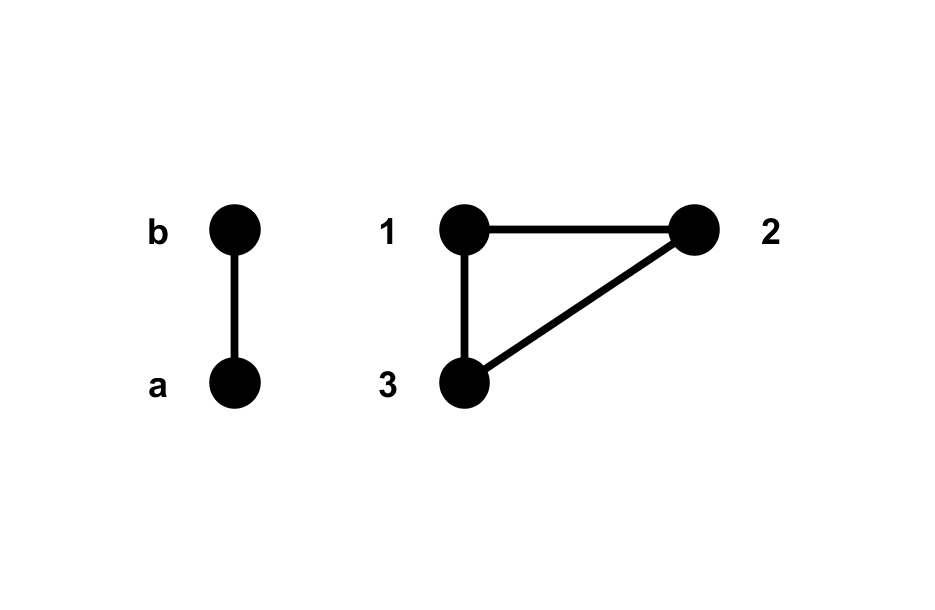
\includegraphics[width=\textwidth]{chapter1/fig/RRWM1}
		\caption{Two graphs to match}
		\label{fig:RRWM1} 
	\end{subfigure}
	~
	\begin{subfigure}[b]{0.33\textwidth}
		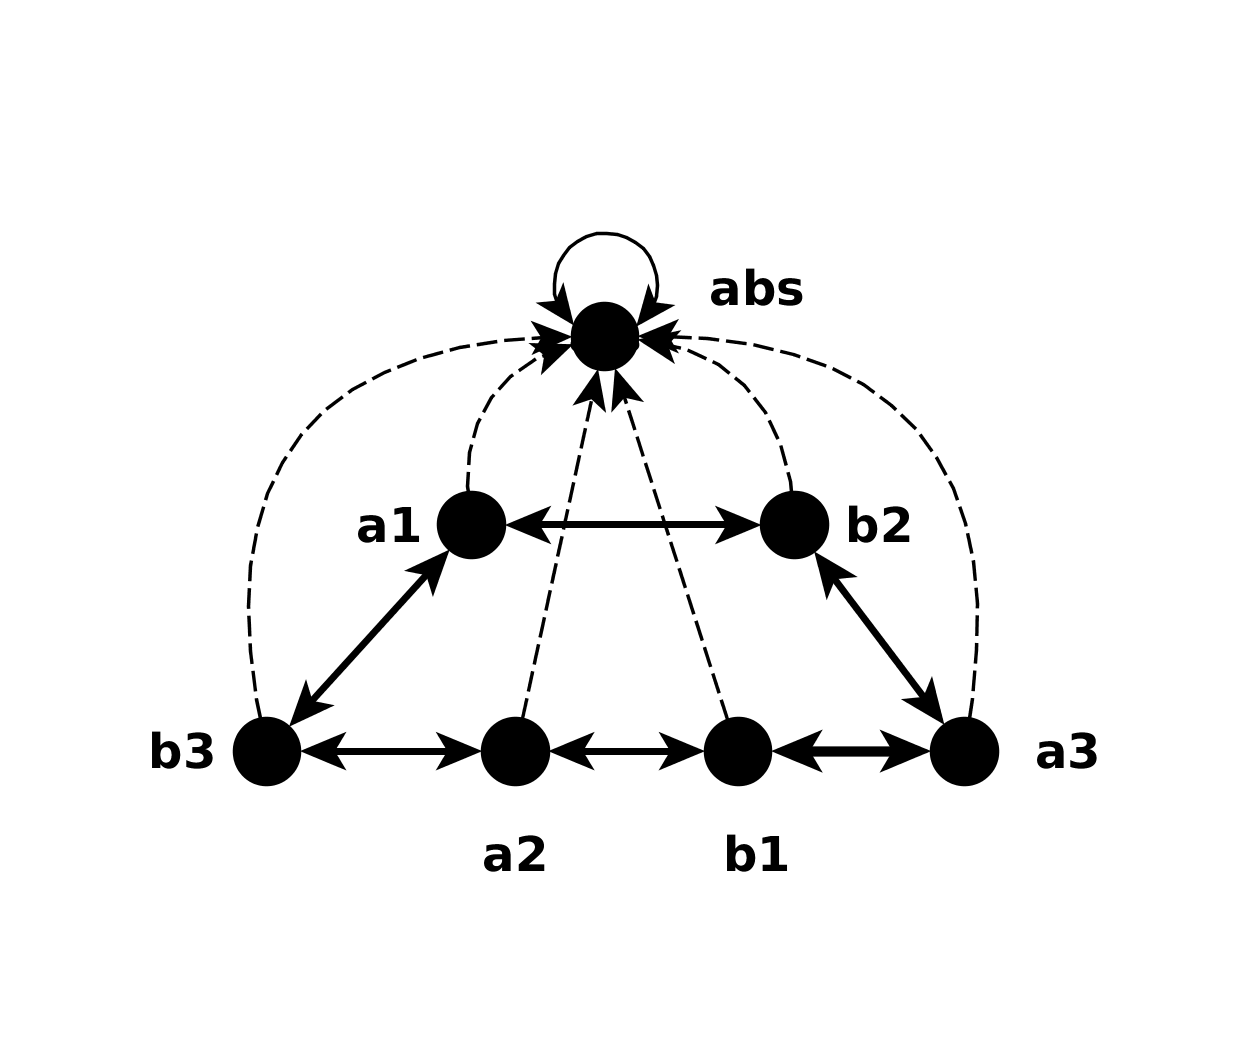
\includegraphics[width=\textwidth]{chapter1/fig/RRWM2}
		\caption{Association graph}
		\label{fig:RRWM2} 
	\end{subfigure}   
	\caption[Association graph in Reweighted Random Walk Method]{Association Graph of two given graphs for Reweighted Random Walk Method (compare with~\cite{Cho2010_RRWM})}
\end{figure}
%\vspace{-10pt}
It is obvious, that the graph matching problem between two graphs $G^I$ and $G^J$ is equivalent to finding a subset of nodes in the associated graph $G^{rw}$, so that the respective node correspondences between $V^I$ and $V^J$ satisfy the matching criteria of the initial problem.
For finding such a subset the authors adopt the page ranking algorithm based on a random walk, which is assumed to be a Markov chain~\cite{PageRank}. To describe a Markov chain one defines a transition matrix $P$. A usual approach to define a transition matrix of a weighted graph $G^{rw}$ is to convert the weighted adjacency matrix $W$ of the graph into a stochastic matrix by the following normalization $P=D^{-1}W$, where $D$ is a diagonal matrix with entries $D_{kk}=\sum_{l}{W_{kl}}$. This method was, for example, used in the PageRank algorithm~\cite{PageRank}. It is however not suitable for the graph matching purposes, as it treats false correspondences equal to all other correspondences. To avoid this problem Cho et al. introduced an additional absorbing node $v_{abs}$~(see Fig.~\ref{fig:RRWM2}) in the Graph $G^{rw}$. This node represents a state, that can be reached from each node $v_k=v_{ij}\in V^{rw}$ with the probability $1-D_{kk}/D_{\text{max}},\ D_{\text{max}}=max_{k}D_{kk}$. Once reached the node  $v_{abs}$ cannot be left any more. Using $D_\text{max}$ the matrix $W$ is converted into a stochastic matrix by its multiplication with the factor $1/D_{\text{max}}$.
Summarizing the transition matrix $P\in\mathbb{R}^{(n_1n_2+1)\times(n_1n_2+1)}$ is defined as 
\begin{equation}P=
\begin{pmatrix}
W/D_{\text{max}} & \mathbf{1}-d/D_{\text{max}} \\
0\dots 0 & 1
\end{pmatrix} \label{eq:RRW_P}
\end{equation}
and update formula of the probability distribution of the Markov chain is defined as
\begin{equation}\label{eq:RRW_MC}
\left(x^{(n+1)T},\ x_{\text{abs}}^{(n+1)}\right)=\alpha\left(x^{(n)T},\ x_{\text{abs}}^{(n)}\right)P+(1-\alpha)r^T,
\end{equation}
where $\mathbf{1}$ in~\eqref{eq:RRW_P} denotes a vector of size $\mathbb{R}^{n_1n_2\times 1}$ with all entries equal to $1$, $d=(D_{11},\dots,D_{n_1n_2})$ is the diagonal of the matrix $D$, $\alpha$ is a weighted factor and $r\in\mathbb{R}^{n_1n_2+1}$ is a \emph{reweighted jump vector}.

A Markov chain, defined by Eq.~\eqref{eq:RRW_MC} without the second term, is denoted by the authors as an \emph{affinity-preserving random walk}. The distribution $\mathbf{\bar{x}}$ of unabsorbed random walks at time $n$ is defined as follows:
\begin{equation}\label{eq:RRWM_x}
\mathbf{\bar{x}}^{(n)}_{ij}=P(X^{(n)}=v_{ij}|X^{(n)}\not=v_{\text{abs}})=\frac{x^{(n)}_{ij}}{1-x^{(n)}_{\text{abs}}}, 
\end{equation}

where $X^{(n)}$ is the current location of a random walker at time $n$. The authors call $\mathbf{\bar{x}}$ a \emph{quasi-stationary distribution} of the absorbed Markov chain. They proof, that the distribution $\mathbf{\bar{x}}$ is proportional to the left principal eigenvector of $W$ and can be efficiently computed with the power iteration method~\cite{PowerIteration}.

The second summand in Eq.~\eqref{eq:RRW_MC} represents the possibility of a random walker to make a jump with probability $(1-\alpha)$ into some constrained node, instead of following the edge. This term was proposed by the authors based on a personalization approach for web page ranking~\cite{Langville2003} as a way to include the matching constraints~\eqref{eq:gQAP3},~\eqref{eq:gQAP4} into random walk. The authors are pointing out, that without this term the matching constraints are incorporated only in the last discretization step of the algorithm, which leads to a weak local maximum. 

A procedure of generation the jump vector $r$ from a current quasi-stationary distribution $\mathbf{\bar{x}}$ consists of two steps. In the first step (\emph{inflation}) unreliable correspondences (i.e. small values in the vector $\mathbf{\bar{x}}$) are damped and the good correspondences are boosted at the same time. The second step (\emph{bistochastic normalization}) forces the matching constraints by transforming the matrix form of $\mathbf{\bar{x}}$ into a double stochastic matrix using the normalization scheme of Sinkhorn~\cite{Sinkhorn1964}. 

\begin{algorithm}[t] 
	\KwIn{ weight matrix $W$, the reweight factor $\alpha$, the inflation factor $\beta$}
	\KwOut{distribution $\mathbf{x}$}
	set $W_{ij,i^\prime j^\prime}$=0 for all conflicting match pairs, i.e. $(v_{ij},v_{ij^\prime})$ and $(v_{ij},v_{i^\prime j})$ \\
	$D_{\text{max}}=\max_{ij}\sum_{i^\prime j^\prime}W_{ij,i^\prime j^\prime}$ \\
	$P=W/D_{\text{max}}$, initialize starting probability $\mathbf{x}$ as uniform\\
	\Repeat{$\mathbf{x}$ converges}{ 
		\tcc{Affinity preserving random walking by edges}
		\nl $\mathbf{\bar{x}}=\mathbf{x}^TP$ \label{alg:Alg1_PowerInteration}\\ 
		\tcc{Reweighting with two-way constraints}
		\tcc{step $1$ inflation:}
		$\mathbf{y}^T=\exp(\beta\mathbf{\bar{x}}/\max\mathbf{\bar{x}})$\\
		\tcc{step $2$ bistochastic normalization :}
		\Repeat{$\mathbf{y}$ converges\label{alg:Alg1_BistochNorm1}}
		{ normalize across rows by $\mathbf{y}_{ij}=\mathbf{y}_{ij}/\sum_{j}\mathbf{y}_{ij}$ \\
			normalize across columns by $\mathbf{y}_{ij}=\mathbf{y}_{ij}/\sum_{i}\mathbf{y}_{ij}$
		}\label{alg:Alg1_BistochNorm2}
		$\mathbf{y}=\mathbf{y}/\sum\mathbf{y}_{ij}$ \\
		\tcc{Affinity-preserving random walking with reweighted jumps}
		$\mathbf{x}^T=\alpha\mathbf{\bar{x}}^T+(1-\alpha)\mathbf{y}^T$ \\
		$\mathbf{x}=\mathbf{x}/\sum\mathbf{x}_{ij}$
	}		
	discretize $\mathbf{x}$ by the matching constraints \label{alg:Alg1_Discr} \\
	\caption{Reweighted Random Walks Method, compare to~\cite{Cho2010_RRWM}}    
	\label{alg:RRWM}
\end{algorithm}

The described steps are summarized in Algorithm~\ref{alg:RRWM} below. The discretization step in line~\ref{alg:Alg1_Discr} can be done by using any method, which solves the linear assignment problem, i.e. the Hungarian algorithm~\cite{Kuhn1955} or greedy heuristic as in~\cite{Leordeanu2005_SM}.

There are some similarities between RRWM and some algorithms, described in chapter~\ref{chapter:GM}. For example, the authors notice, that line~\ref{alg:Alg1_PowerInteration} of Algorithm~\ref{alg:RRWM} can be considered as the power iteration version of SM~\cite{Leordeanu2005_SM}. Also the Sinkhorn normalization (line~8-\ref{alg:Alg1_BistochNorm2}) was used in soft-assign step in~\cite{Rangarajan1996_GAGM}. 

%In the chapter~\ref{chapter:results} we discuss experimental results of the RRWM for graph matching.

The complexity of the algorithm is $\mathcal{O}(|E^I||E^J|)$ per iteration, whereby the quasi-stationary distribution $\mathbf{\bar{x}}$ in line~\ref{alg:Alg1_PowerInteration} was computed with the power iteration method~\cite{PowerIteration}.

